
\documentclass[twoside,letterpaper,12pt]{report}
\usepackage{aux/samstyle}

\author{
Sergio Andrés Monsalve Castañeda \\
smonsal3@eafit.edu.co\\
Departamento de Informática y Sistemas \\[1cm]
Presentado a:\\
Maria Eugenia Puerta Yepes\\[0.2cm]
Matemática Aplicada\\
Departamento De Ciencias Matemáticas\\
Universidad EAFIT\\[3cm] 
Copyright \copyright \hspace{3pt} Universidad EAFIT 2015
}

\title{ \textbf{Modelo Matemático\\ Predicción de Dengue}\\
Documento de Requisitos\\
}

\date{\today}
%\includeonly{tex/arte,tex/intro}

\begin{document}
\maketitle

\tableofcontents

\pagestyle{fancyplain}
\fancyhf{}
\headheight=30pt %para cambiar el tamaño del encabezado
\renewcommand{\headrulewidth}{0pt} %espesor del encabezado

\lhead %la "L" indica a la izquierda
{
\begin{minipage}{2cm}

\includegraphics[width=1.5 in]{aux/Logo_EAFIT.jpg}
\end{minipage}
}

\fancyfoot[c]{\thepage}

\begin{abstract}
El presente documento pretende proporcionar un listado de las espectativas del Cliente y el Usuario Final.
Cliente: Departamento de Matematica Aplicada 
Usuario Final: Medico Epidemiologo
\end{abstract}

\section{Actividades de la Semana}


\begin{itemize}

\item Analisis de Requisitos Inicial

\item Documento Requisitos Funcionales y No Funcionales

\item Revisión herramientas de Georeferenciación

\item Revisión herramientas de Desarrollo 

\item Busqueda de 

\item Creación de Repositorio en Github

\item Documentación Inicial

\item Cronograma de Actividades

\item Presentación Paola Lizarralde Predefensa de Tesis en el SIU

\item Desarrollo de Informe

\item Lectura artículo de Referencia\cite{scavuzzoalgoritmos}

\end{itemize}
 
\chapter{Requisitos Funcioanles}


los siguientes elementos mapean a los componentes  correspondientes a como se espera debe funcionar el Sistema

\begin{itemize}
	\item Caputar Entradas Año Epidemiologico- Semanas- Casos
	\item Canal Endémico
		\begin{itemize}
			\item Calculo modelo Ecuaciónes Diferenciales
			\item Alerta 
		\end{itemize}
	\item Georeferenciación
	\item Mapas de calor según numero de casos por zona
	\item Consultas

\end{itemize}

\chapter{Requisitos No Funcionales}


los siguientes elementos mapean a los atributos de Calidad correspondientes a los requisitos no Funcionales del Sistema

\begin{figure}[h]
\begin{center}
  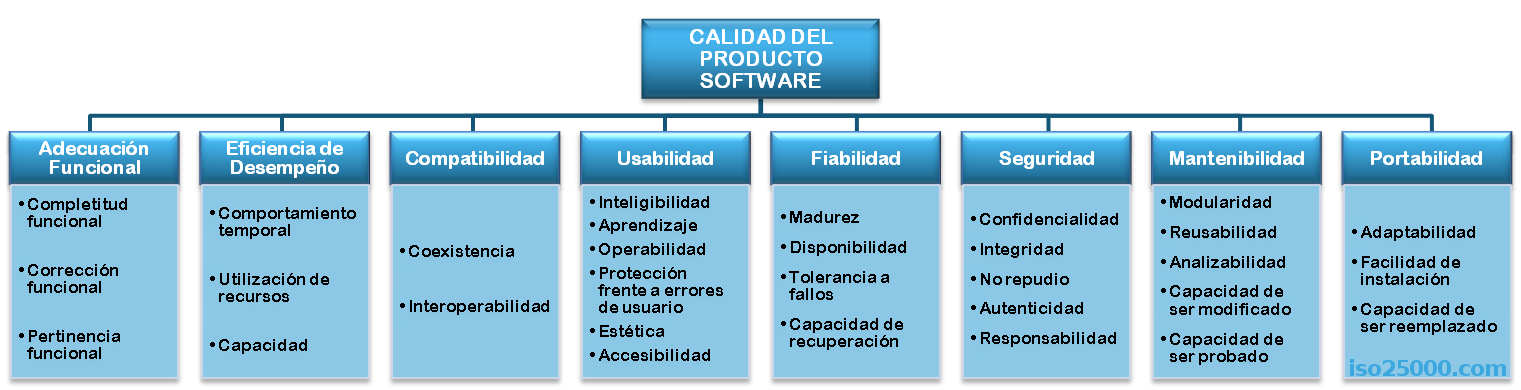
\includegraphics[width=\textwidth]{aux/nofun}
  \caption{Requisitos No funcionales}
  \label{figCasosUso}
\end{center}
\end{figure}

\begin{itemize}
	\item Seguridad
	\item Autenticación
	\item Autorización
		\begin{itemize}
			\item Definición de Roles
		\end{itemize}
	\item Disponibilidad
	\item Usabilidad
	\item Modificabilidad
	\item Testeabilidad
\end{itemize}

\bibliographystyle{ieeetr}
\bibliography{aux/refs}

\appendix
\chapter{Notas}

%\todo[inline,caption={TODO}]{To - do}

\end{document}
